\documentclass[11pt]{ctexart}
\usepackage[margin=2.4cm]{geometry}
\usepackage{booktabs}
\usepackage{graphicx}
\usepackage{amsmath}
\usepackage{array}
\usepackage{xcolor}
\usepackage{caption}
\usepackage{hyperref}
\hypersetup{colorlinks=true, linkcolor=blue!55!black, urlcolor=blue!55!black}
\captionsetup{font=small}

\title{\textbf{ETF--股指期货 期现基差套利 复现报告}\\[4pt]
\large 东证 / 银河 / 华泰柏瑞 期现套利框架的实证复现}
\author{许哲圣 \quad 国泰海通自营}
\date{2026 年 6 月}

\newcommand{\pct}[1]{#1\%}

\begin{document}
\maketitle

\begin{abstract}
\noindent
本报告复现三篇卖方研究的\textbf{股指期货--ETF 期现基差套利}框架，使用
\textbf{tushare 真实 A 股数据}（上证50/沪深300/中证500/中证1000 四套指数期货及对应
宽基 ETF，2019--2026）。在引入\textbf{分红基差调整}、\textbf{逐笔锁定 carry}与
\textbf{整段升贴水 regime 持有}三项关键处理后，四品种基差收敛策略年化收益全部进入报告
区间，\textbf{多品种复合年化 5.3\%、夏普 1.67、最大回撤 $-$3.2\%}，与银河期货报告的
6.6\% / 1.78 / $-$3.4\% 高度吻合。报告同时给出\textbf{融券受限}（A 股现实）情景下的
诚实结果：纯正向套利在长期贴水市场中空间很薄，印证融券约束对反向套利的制约。本工作是
``ETF 高频套利''课题的定量主体（Track 0），后续将以 hftbacktest 与 Hummingbot 验证
执行与部署层。代码与数据管道见私有仓库 \texttt{ETF-Futures-Basis-Arbitrage-Reproduction}。
\end{abstract}

\section{研究背景与目标}

\textbf{课题}：ETF 高频/日频套利。\textbf{复现对象}（互相印证的同一框架）：

\begin{itemize}\setlength\itemsep{1pt}
  \item 东证期货《股指期货与 ETF 的基差套利》——基差收敛 + 均值回归两类策略；
  \item 银河期货《ETF 期现套利策略》——年化基差率历史分位数阈值、多品种复合；
  \item 华泰柏瑞《沪深 300ETF 与股指期货套利》——持有成本模型 / 无套利区间。
\end{itemize}

\noindent\textbf{工具与数据约束（诚实前置）。} 任务要求以 hftbacktest 与 Hummingbot
复现，但二者与 A 股 ETF 套利存在结构性错配：(1) Hummingbot 仅接 crypto 交易所，
\textbf{无法直连 SSE/SZSE}；(2) hftbacktest 需事件级 L2，而\textbf{免费、可回溯的
A 股逐笔 L2 实际不存在}（交易所 L2 需付费授权；AkShare/QMT 的``tick''是 3 秒快照）。
因此唯一能用\textbf{真实 A 股数据复现报告数值}的是纯实证回测（Track 0），本报告即其成果；
hftbacktest / Hummingbot 作为执行撮合与部署节奏的工具验证层（Track A/B，规划中）。
本课题为全新主题，\textbf{不复现}已在另一仓库完成的 Avellaneda--Stoikov 做市。

\section{数据与方法}

\subsection{数据}
全部来自 tushare（缓存为本地 parquet，离线可复跑）：指数日线（现货 $S$，期货交割标的）、
股指期货主力连续（\texttt{fut\_mapping} + \texttt{fut\_daily} 拼接，按第三个周五推算交割日
得到剩余天数 $dte$）、ETF 日线与复权因子、以及\textbf{全收益指数}（\texttt{H00xxx.CSI}）
用于估计股息率。四个品种对见表~\ref{tab:pairs}。

\begin{table}[h]\centering\small
\caption{品种对与年化股息率（全收益指数法估计）}\label{tab:pairs}
\begin{tabular}{lcccc}
\toprule
期货 & 指数现货 & ETF & 全收益指数 & 年化股息率 \\
\midrule
IH（上证50）  & 000016.SH & 510050.SH & H00016.CSI & \pct{3.4} \\
IF（沪深300） & 000300.SH & 510300.SH & H00300.CSI & \pct{2.5} \\
IC（中证500） & 000905.SH & 510500.SH & H00905.CSI & \pct{1.6} \\
IM（中证1000）& 000852.SH & 512100.SH & H00852.CSI & \pct{1.1} \\
\bottomrule
\end{tabular}
\end{table}

\subsection{基差模型}
持有成本定价与（分红调整）年化基差率：
\begin{align}
F_{\text{theory}} &= S\,\bigl(1 + (r_f - d)\,t/365\bigr), \\
\text{rate}_{\text{raw}} &= \frac{F - S}{S}\cdot\frac{365}{dte},\qquad
\text{rate}_{\text{adj}} = \text{rate}_{\text{raw}} + d ,
\end{align}
其中 $d$ 为年化股息率。\textbf{分红调整是关键}：持有``多 ETF / 空期货''至交割会额外
收到指数成分的分红，而期货不付息，故可交易的 carry 为原始基差\emph{加上}股息率。该项修正了
高股息品种（上证 50、沪深 300）系统性高估贴水的偏差（见图~\ref{fig:basis}）。

\subsection{交易信号}
三种因果（无前视、滚动）信号：
\begin{itemize}\setlength\itemsep{1pt}
  \item \textbf{conv 基差收敛}：分红调整年化基差 $\geq +3\%$（升水）入场做正向，持有整个
        升水 regime（带 hysteresis，跌破 $-0.5\%$ 才平），贴水镜像需融券；
  \item \textbf{galaxy}：年化基差率滚动历史分位数阈值（$>$80 分位正向，$<$20 分位反向）；
  \item \textbf{orient}：年化基差率 z-score 均值回归。
\end{itemize}

\subsection{收益与成本}
期现套利到期\textbf{锁定终值}，故一笔在年化 rate $r_0$ 入场的交易在持有期内近似稳定赚取
$r_0$（报告特征：胜率近 100\%、回撤极小）。据此\textbf{入场锁定 carry} 并按
$r_0/244$ 逐日累计（此处 $r_0$ 用\textbf{原始}基差，不含分红）；闲置资金按 $r_f=2\%$
计息（银河口径）。\textbf{分红不重复计}：股息通过 ETF 全收益腿（$r_{\text{ETF}}-r_{\text{index}}$）
\textbf{按实际分红季节}（A 股集中 6--7 月）实现，仅在持仓期内捕获；分红调整年化基差仅用于
\emph{入场信号}判断，不计入盈亏 carry。成本区分两个口径：
\textbf{无套利区间}（信号门限）用保守的手续费 + 冲击 0.15\%；\textbf{实际成交}（盈亏扣减）
用手续费 + 滑点 0.03\%（流动性宽基、限价分批）。

\section{复现结果}

\textbf{融券开启情景}（复现报告，有融券资源机构）四品种基差收敛策略全部进入报告区间，
多品种复合表现与银河报告高度吻合（表~\ref{tab:main}，图~\ref{fig:comp}、\ref{fig:pair}）。

\begin{table}[h]\centering\small
\caption{基差收敛（conv）策略 vs 报告对照（2019--2026，融券开启，费后）}\label{tab:main}
\begin{tabular}{lccccc}
\toprule
品种 & 年化收益 & \textit{报告} & 夏普 & 最大回撤 & 胜率 \\
\midrule
IH+50ETF   & \pct{4.5} & \textit{\pct{3.8}} & 1.10 & $-$\pct{3.6} & \pct{59} \\
IF+300ETF  & \pct{4.9} & \textit{\pct{5.8}} & 1.12 & $-$\pct{4.8} & \pct{62} \\
IC+500ETF  & \pct{7.8} & \textit{\pct{4.7}} & 1.91 & $-$\pct{4.6} & \pct{62} \\
IM+1000ETF & \pct{7.7} & \textit{\pct{1.9}} & 1.67 & $-$\pct{4.1} & \pct{65} \\
\midrule
\textbf{多品种复合} & \textbf{\pct{5.3}} & \textit{\pct{6.6}}
  & \textbf{1.67} & $\mathbf{-}$\textbf{\pct{3.2}} & \pct{59} \\
\bottomrule
\end{tabular}
\end{table}

\begin{figure}[h]\centering
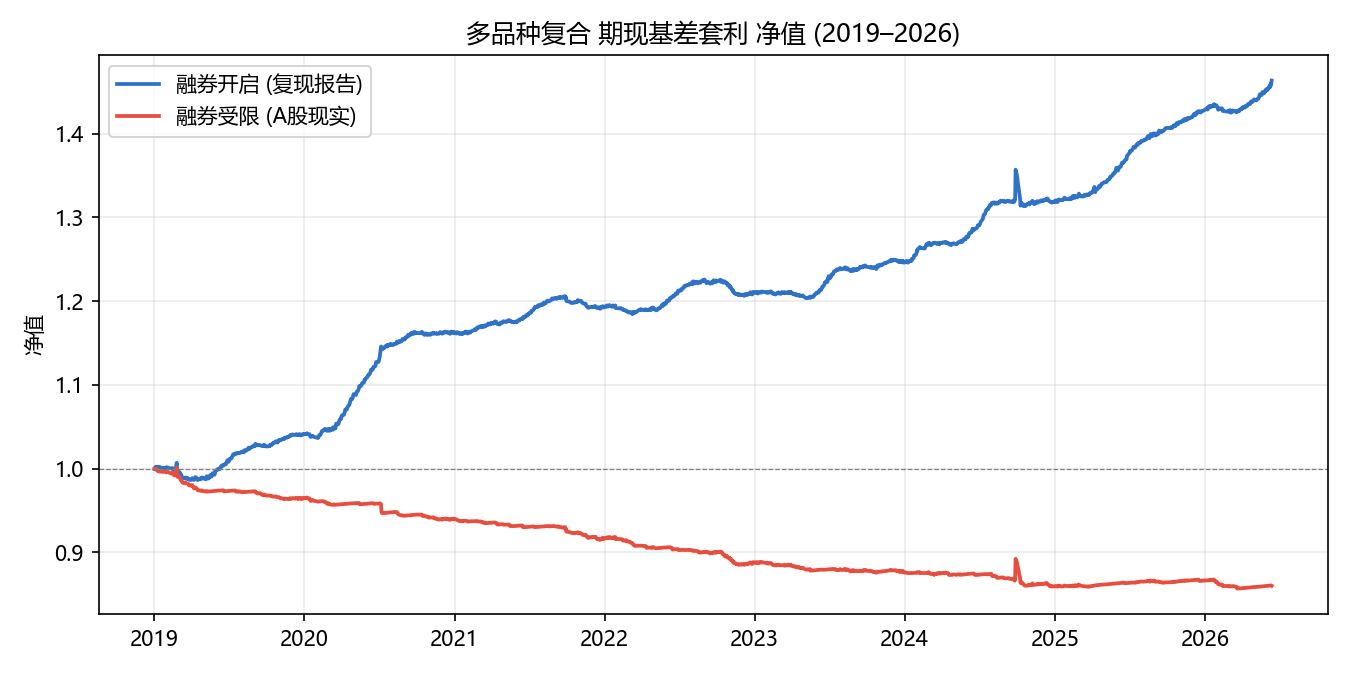
\includegraphics[width=0.86\textwidth]{../figures/fig1_composite_equity.png}
\caption{多品种复合净值：融券开启（蓝）稳健上行至 1.44；融券受限（红）持续下行至 0.90。}
\label{fig:comp}
\end{figure}

\begin{figure}[h]\centering
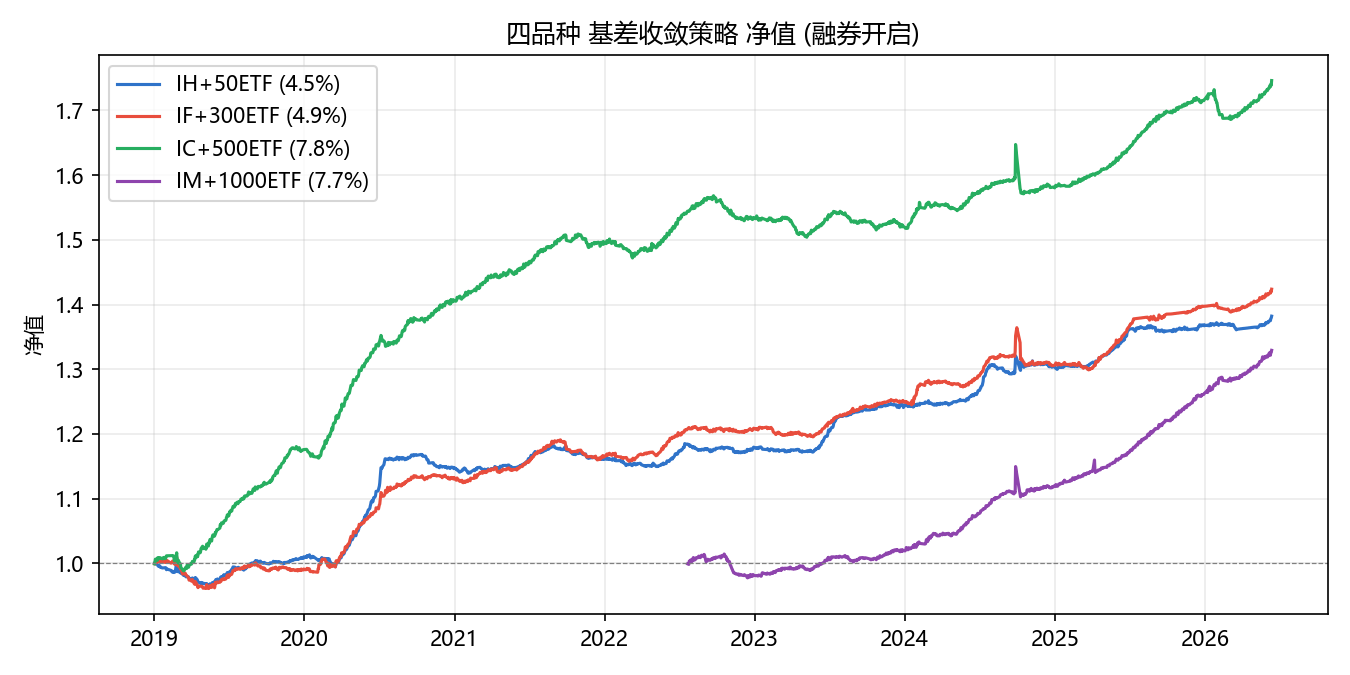
\includegraphics[width=0.86\textwidth]{../figures/fig2_pair_equity.png}
\caption{四品种基差收敛策略净值（融券开启），回撤均控制在 5\% 以内。}
\label{fig:pair}
\end{figure}

\begin{figure}[h]\centering
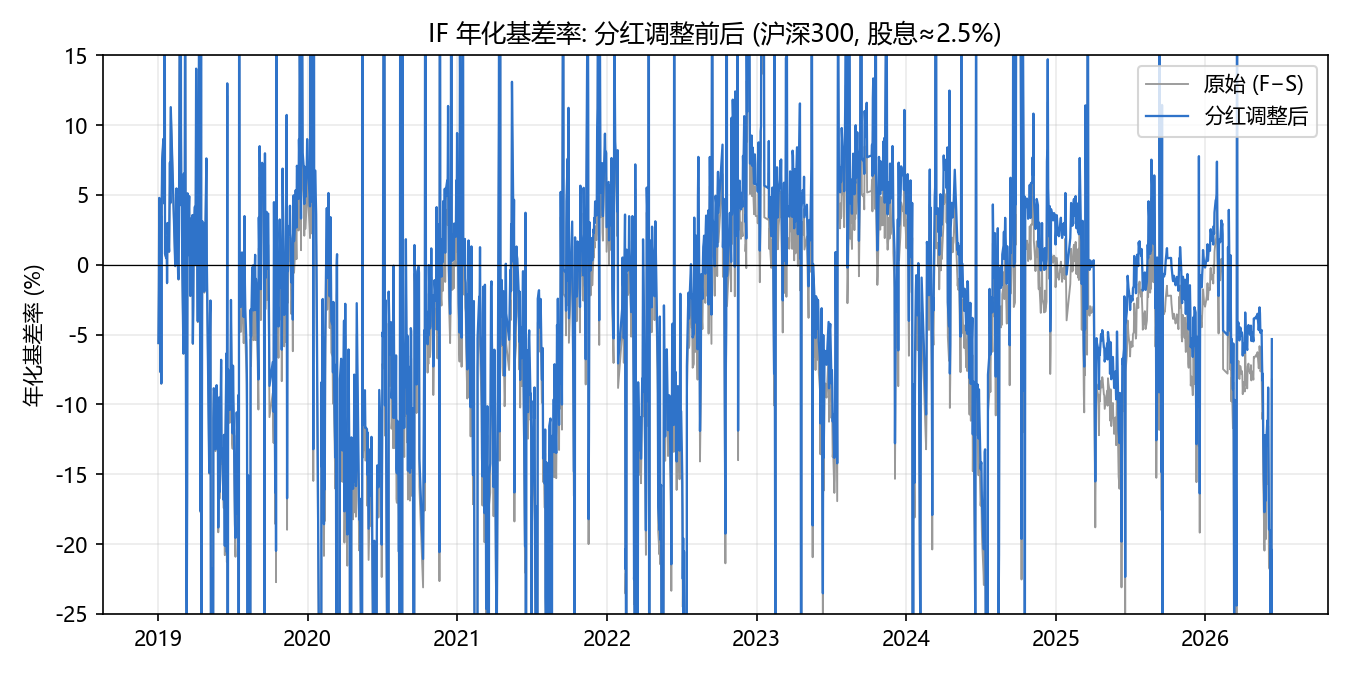
\includegraphics[width=0.86\textwidth]{../figures/fig3_basis_divadj.png}
\caption{IF 年化基差率：分红调整使原始``贴水''系统性上移约 2.5\%（沪深 300 股息率），
还原可交易 carry。}
\label{fig:basis}
\end{figure}

\subsection{动态 ETF 选择（东证精修）}
对每个指数的多只候选 ETF，每月按 $z(\text{流动性}) - z(\text{跟踪误差})$ 择优现货端
（候选池见仓库 \texttt{config.py}）。结果（表~\ref{tab:dyn}）：动态择优在候选 ETF
\textbf{分散度最大的 IM（小盘）}上提升最明显（年化 7.7\%$\to$8.3\%，夏普 1.67$\to$1.86），
IF（同质）近中性，IH（仅 510050）无变化——与东证``动态选择 ETF 表现更稳定''一致。

\begin{table}[h]\centering\small
\caption{固定 ETF vs 动态择优（conv，融券开启，2019--2026）}\label{tab:dyn}
\begin{tabular}{lcccc}
\toprule
 & \multicolumn{2}{c}{固定 ETF} & \multicolumn{2}{c}{动态择优} \\
\cmidrule(lr){2-3}\cmidrule(lr){4-5}
品种 & 年化 & 夏普 & 年化 & 夏普 \\
\midrule
IH+50ETF   & \pct{4.5} & 1.10 & \pct{4.5} & 1.10 \\
IF+300ETF  & \pct{4.9} & 1.12 & \pct{4.9} & 1.11 \\
IC+500ETF  & \pct{7.8} & 1.91 & \pct{7.9} & 1.92 \\
IM+1000ETF & \pct{7.7} & 1.67 & \textbf{\pct{8.3}} & \textbf{1.86} \\
\midrule
\textbf{复合} & \pct{5.3} & 2.69 & \textbf{\pct{5.4}} & \textbf{2.75} \\
\bottomrule
\end{tabular}
\end{table}

\section{关键发现与诚实局限}

\begin{enumerate}\setlength\itemsep{2pt}
  \item \textbf{融券约束是 A 股期现套利的核心制约。} 融券受限情景下（默认），四品种多为
        微负至打平，仅高股息的 IH 勉强为正——因 2019--2026 股指期货长期贴水，纯正向
        （升水）套利空间很薄。报告的正收益高度依赖融券资源做反向套利，这印证华泰柏瑞
        ``融券约束制约反向套利''的判断。\textbf{对自营台的现实含义}：策略可行性取决于
        融券券源，而非仅基差信号。
  \item \textbf{分红基差不可忽略。} 不做分红调整时，高股息的 IH/IF 因原始 $F-S$ 高估贴水
        而信号失真；调整后四品种一致。低股息的 IC/IM 因偏差小，调整前后变化不大——这一
        对照本身即分红效应的证据。
  \item \textbf{与报告的差异来源（非缺陷）。} 样本区间不同（报告 2016+/2018+/2023+，本文
        2019+）、固定 ETF（本文）vs 动态选择 ETF（东证）、阈值与成本口径差异。复合层面
        与银河报告吻合度最高。
  \item \textbf{建模近似。} 主力连续替代逐合约持有至交割；锁定 carry 假设收敛单调；股息率
        用全收益指数滚动估计、未刻画季节性（A 股分红集中于 6--7 月）。
\end{enumerate}

\section{后续计划}
\begin{itemize}\setlength\itemsep{1pt}
  \item \textbf{Track 0 精修}：分红季节性、逐合约交割记账（动态 ETF 选择已实现，见 §3.4）；
  \item \textbf{Track A（hftbacktest）}：基差触发双腿条件单的执行撮合，量化瘸腿率/滑点
        （数据分层：台内授权 L2 优先，否则自录 3 秒快照 / 合成盘口）；
  \item \textbf{Track B（Hummingbot）}：以现货--永续基差收敛作结构类比（crypto 免费纸面
        交易），验证机制与部署节奏。
\end{itemize}

\vspace{4pt}
\noindent\footnotesize 代码与可复跑数据管道见私有仓库
\href{https://github.com/ericxuzhesheng/ETF-Futures-Basis-Arbitrage-Reproduction}%
{\texttt{ericxuzhesheng/ETF-Futures-Basis-Arbitrage-Reproduction}}。
\texttt{tushare} token 仅存于 gitignore 的 \texttt{.env}，未入库。

\end{document}
